% !TeX encoding = UTF-8
% !TeX spellcheck = es_ANY
\documentclass[xcolor=table, t]{beamer}

\usepackage[T1]{fontenc}

\usepackage[spanish]{babel}

\usepackage{amsmath,amssymb,amsfonts,latexsym,amsthm,stmaryrd} 

\usepackage{listings}

\usepackage{xcolor}
\usepackage{hyperref}

\usepackage{cite}
\usepackage{url}
\usepackage{mathtools}

\mathtoolsset{showonlyrefs}

\renewcommand{\Re}{\mathfrak{Re}}
\renewcommand{\epsilon}{\varepsilon}
\newcommand{\R}{\mathbb{R}}
\newcommand{\C}{\mathbb{C}}
\newcommand{\Q}{\mathbb{Q}}
\newcommand{\N}{\mathbb{N}}
\newcommand{\dis}{\displaystyle}
\newcommand{\dem}{{\bf Sobre la demostración:}}
\newcommand{\an}{\bf\color{blue}\bf}

%\usefonttheme{professionalfonts}
%\usetheme{Warsaw}
\setbeamercovered{transparent}

\definecolor{colorcesbio}{RGB}{37, 145, 17}
\definecolor{forestgreen}{rgb}{0.13, 0.55, 0.13}
\definecolor{greenyellow}{rgb}{0.68, 1.0, 0.18}
\definecolor{inchworm}{rgb}{0.7, 0.93, 0.36}

\definecolor{uprgreen}{RGB}{18,104,47}
\definecolor{uprgreen2}{RGB}{51,144,55}

\setbeamercolor{title in head/foot}{bg=uprgreen, fg=uprgreen}
\setbeamercolor{author in head/foot}{bg=uprgreen}
%\setbeamertemplate{page number in head/foot}{}

\useoutertheme{infolines}
\usetheme{Warsaw}
\usecolortheme[named=uprgreen]{structure}

\setbeamercovered{transparent}

\title{Conferencia $\#$5}
\subtitle{Integración Numérica, Aplicaciones y Ejemplos} 
\author{Lic. Alguien Alguien Alguien\ \hfill \href{mailto:alguien.alguien@upr.edu.cu}{alguien.alguien@upr.edu.cu}}
\date{Departamento de Matemática}

\begin{document}
	\frame{\titlepage
	\begin{center}
		
\includegraphics[height=2.5cm]{img/cortado.png}
	\end{center}
	}
	\begin{frame}
		\ \\ \ \\
		\begin{block}{}
			Uno de los problemas más antiguos es el cálculo de áreas. En particular el del círculo, el cuál tuvo una solución muy elegante mediante la cuadratura del círculo.
		\end{block}
	\end{frame}
	\begin{frame}
		\ \\ \ \\
		\begin{block}{}
			Uno de los problemas más antiguos es el cálculo de áreas. En particular el del círculo, el cuál tuvo una solución muy elegante mediante la cuadratura del círculo.
		\end{block}
		\begin{center}
			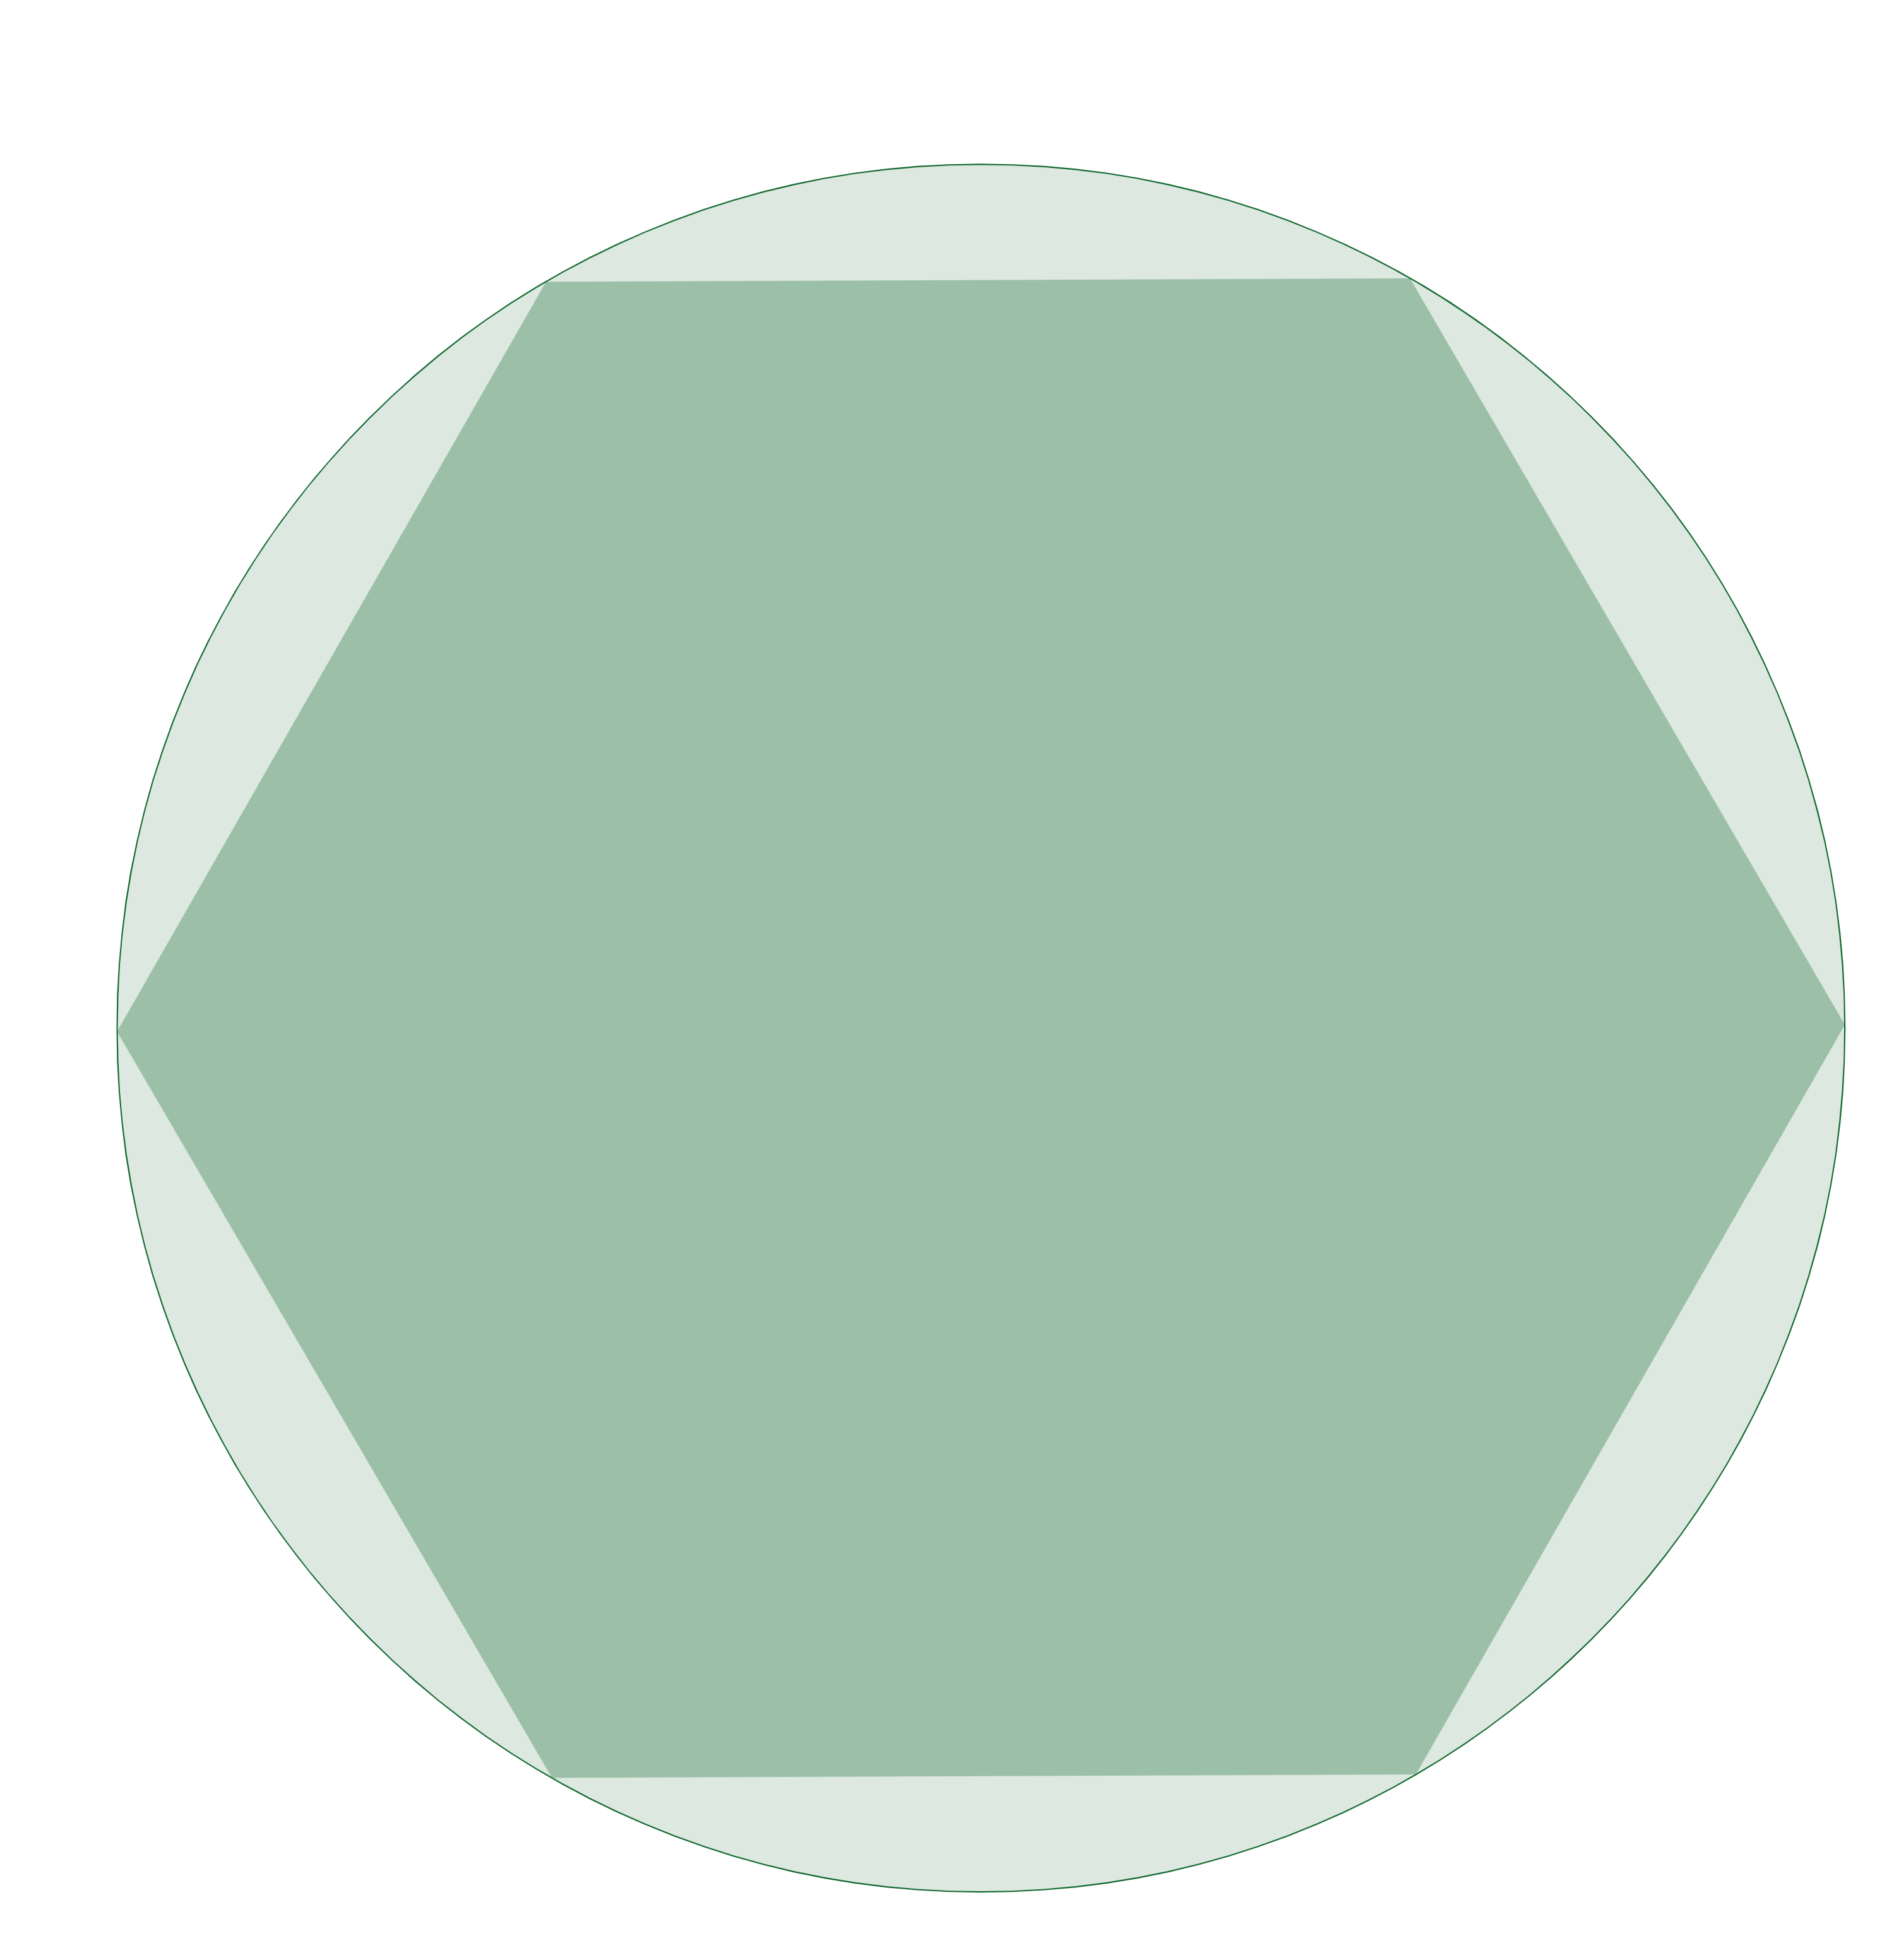
\includegraphics[height=5cm]{img/fig1.png}
		\end{center}
	\end{frame}
	\begin{frame}
		\ \\ \ \\
		\begin{block}{}
			Uno de los problemas más antiguos es el cálculo de áreas. En particular el del círculo, el cuál tuvo una solución muy elegante mediante la cuadratura del círculo.
		\end{block}
		\begin{center}
			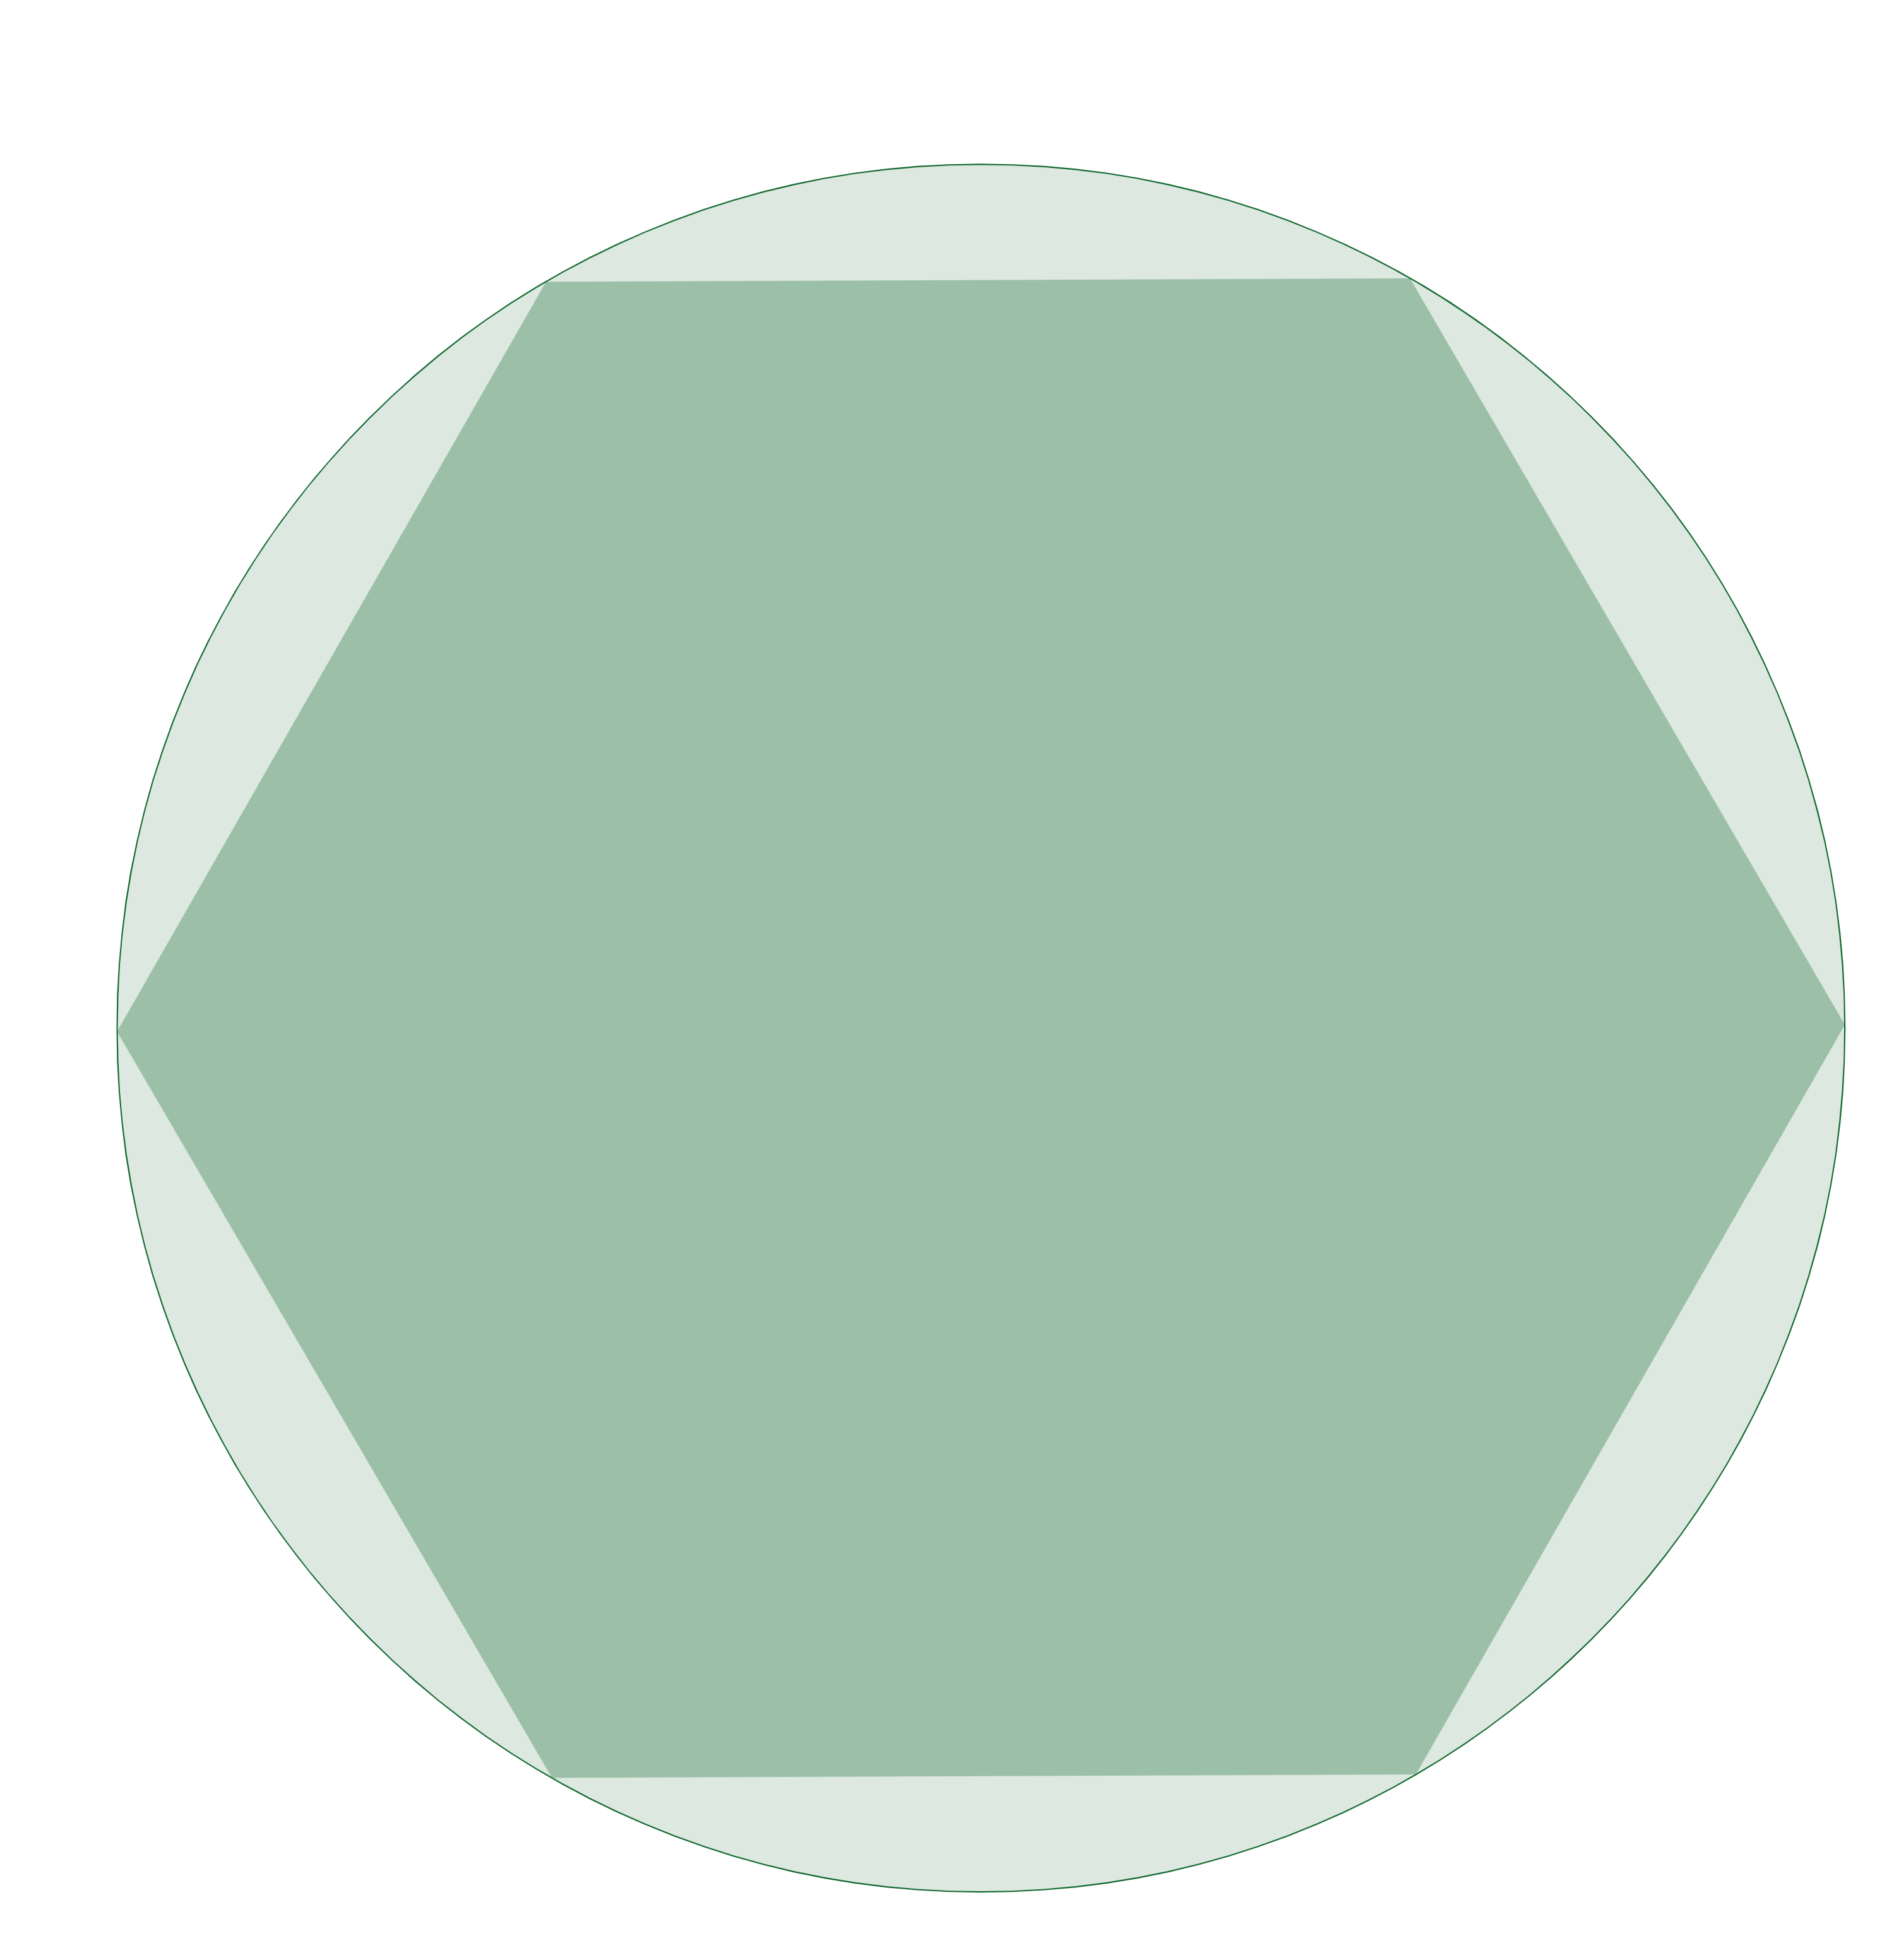
\includegraphics[height=5cm]{img/fig1.png}
			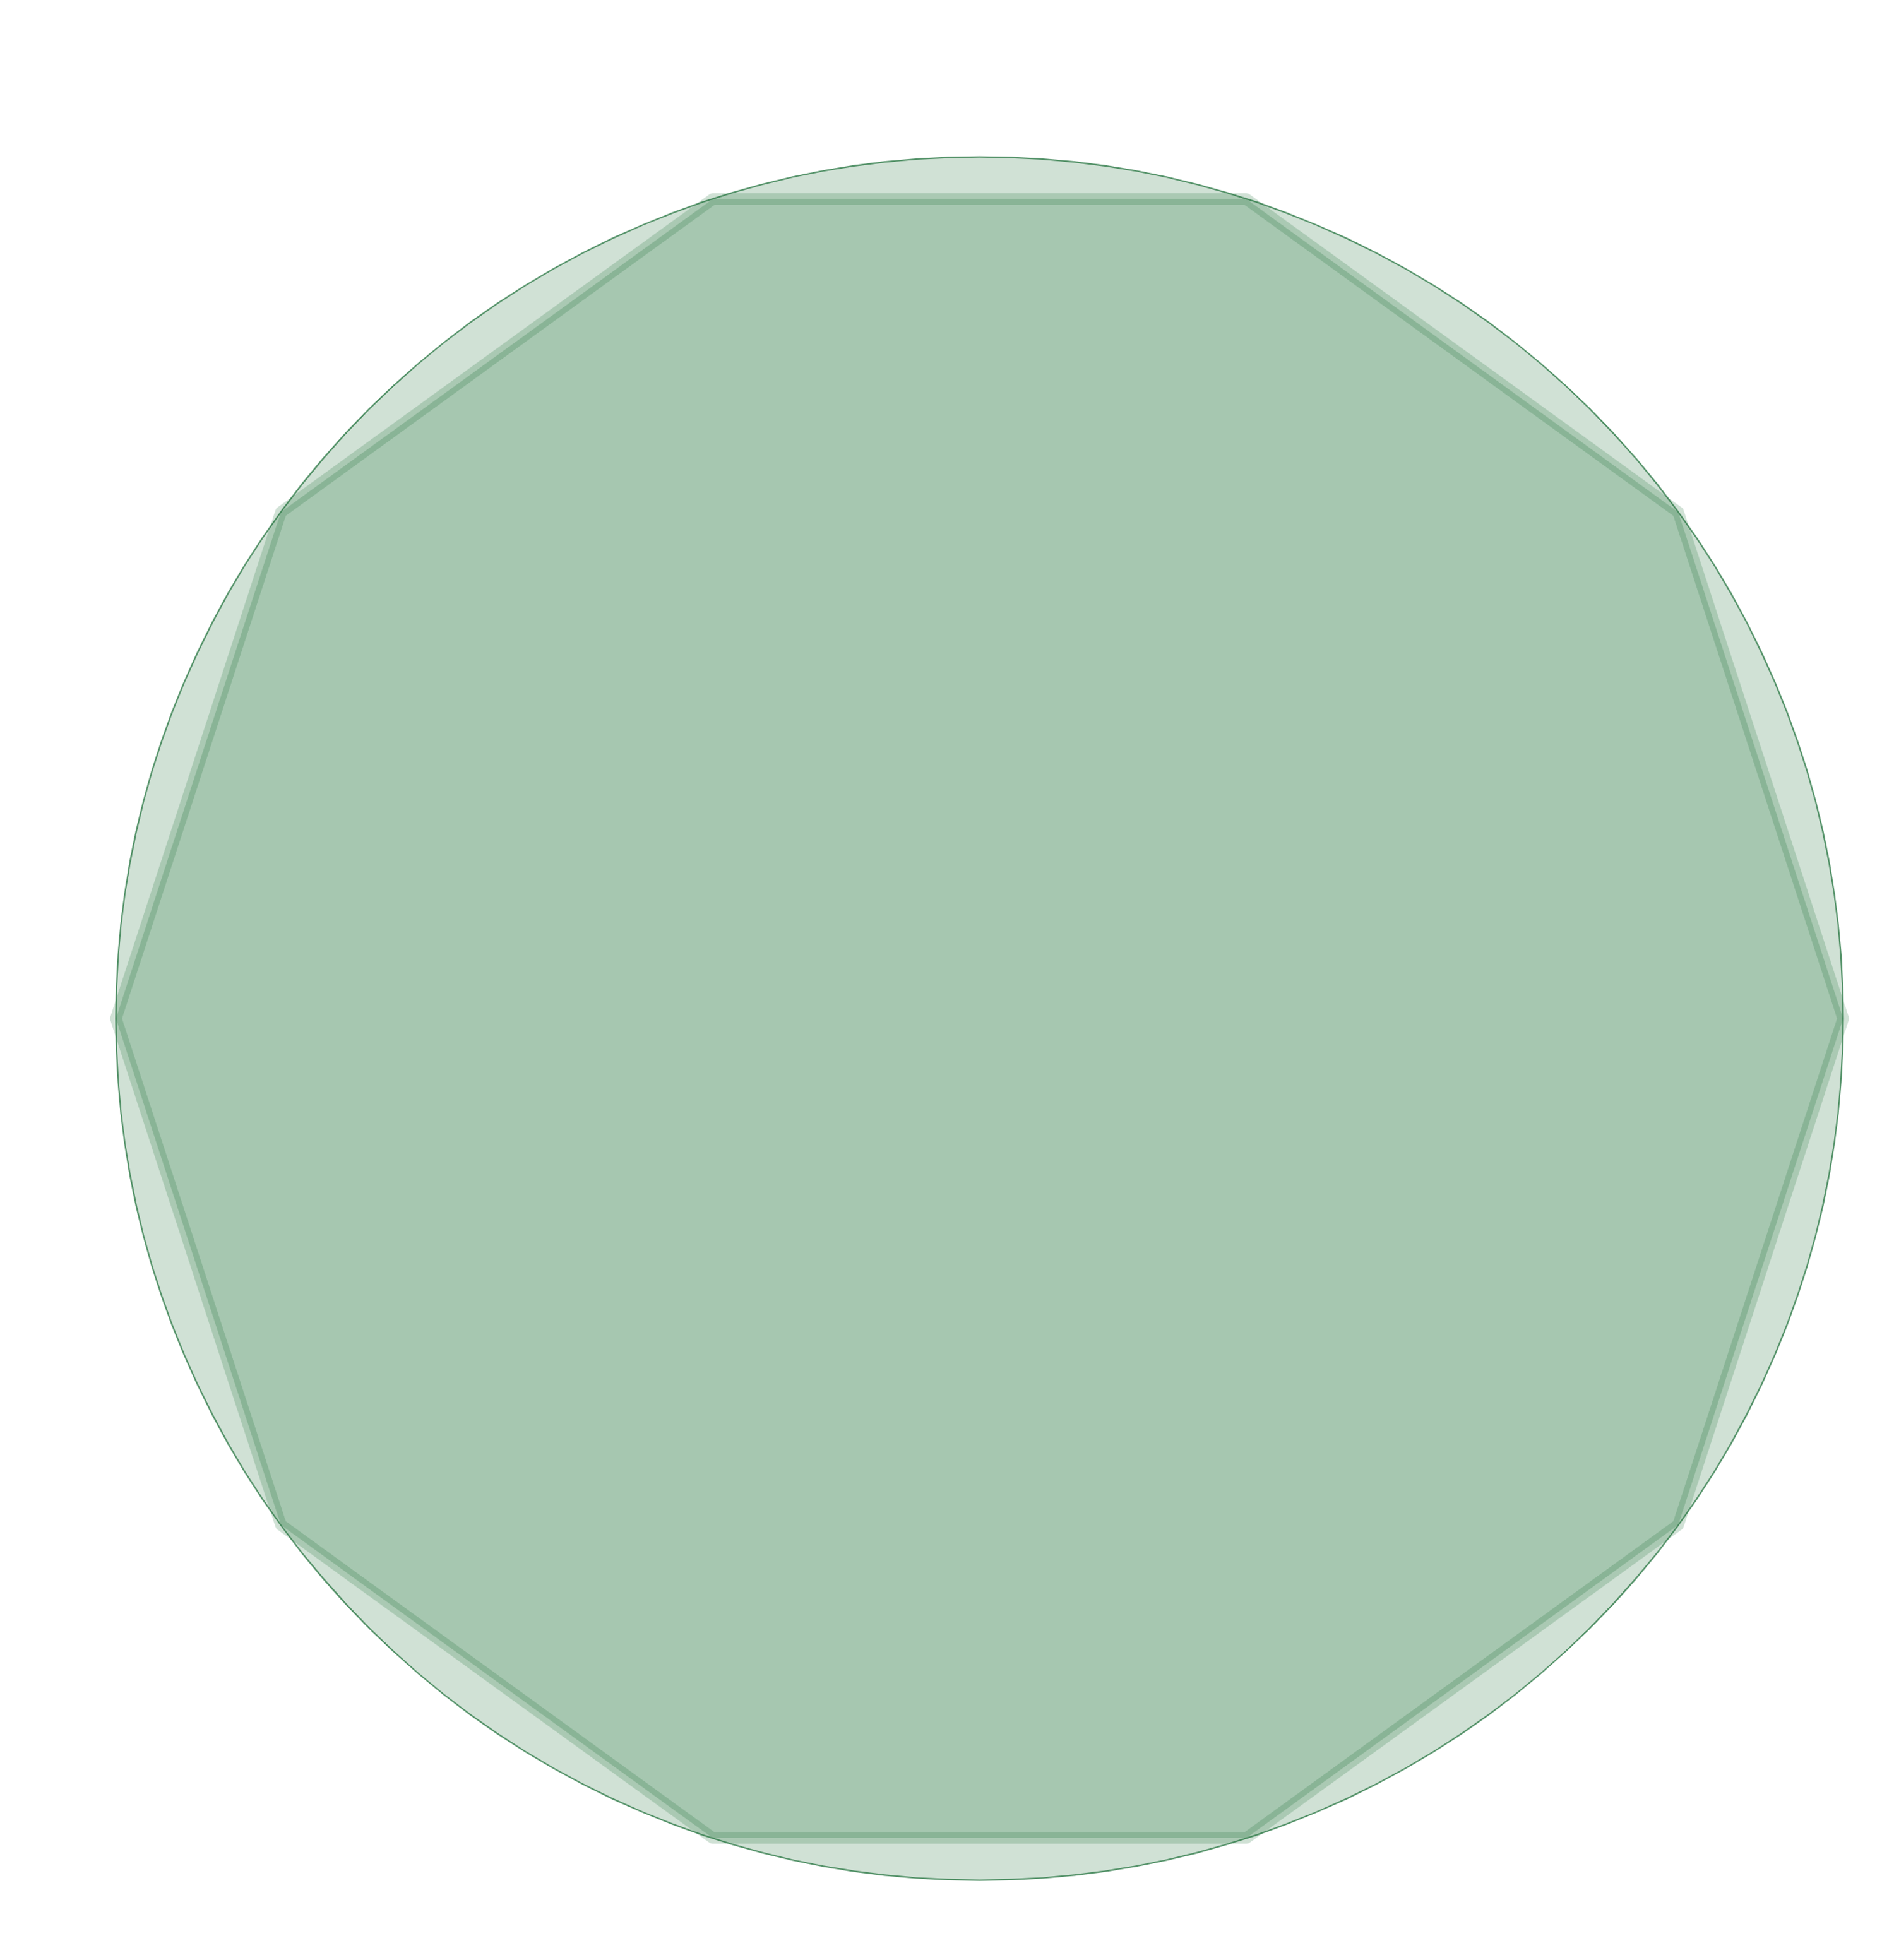
\includegraphics[height=5cm]{img/fig2.4.png}
		\end{center}
	\end{frame}
	\begin{frame}
		\begin{block}{}
			Uno de los problemas más antiguos es el cálculo de áreas. En particular el del círculo, el cuál tuvo una solución muy elegante mediante la cuadratura del círculo.
		\end{block}
		\begin{center}
			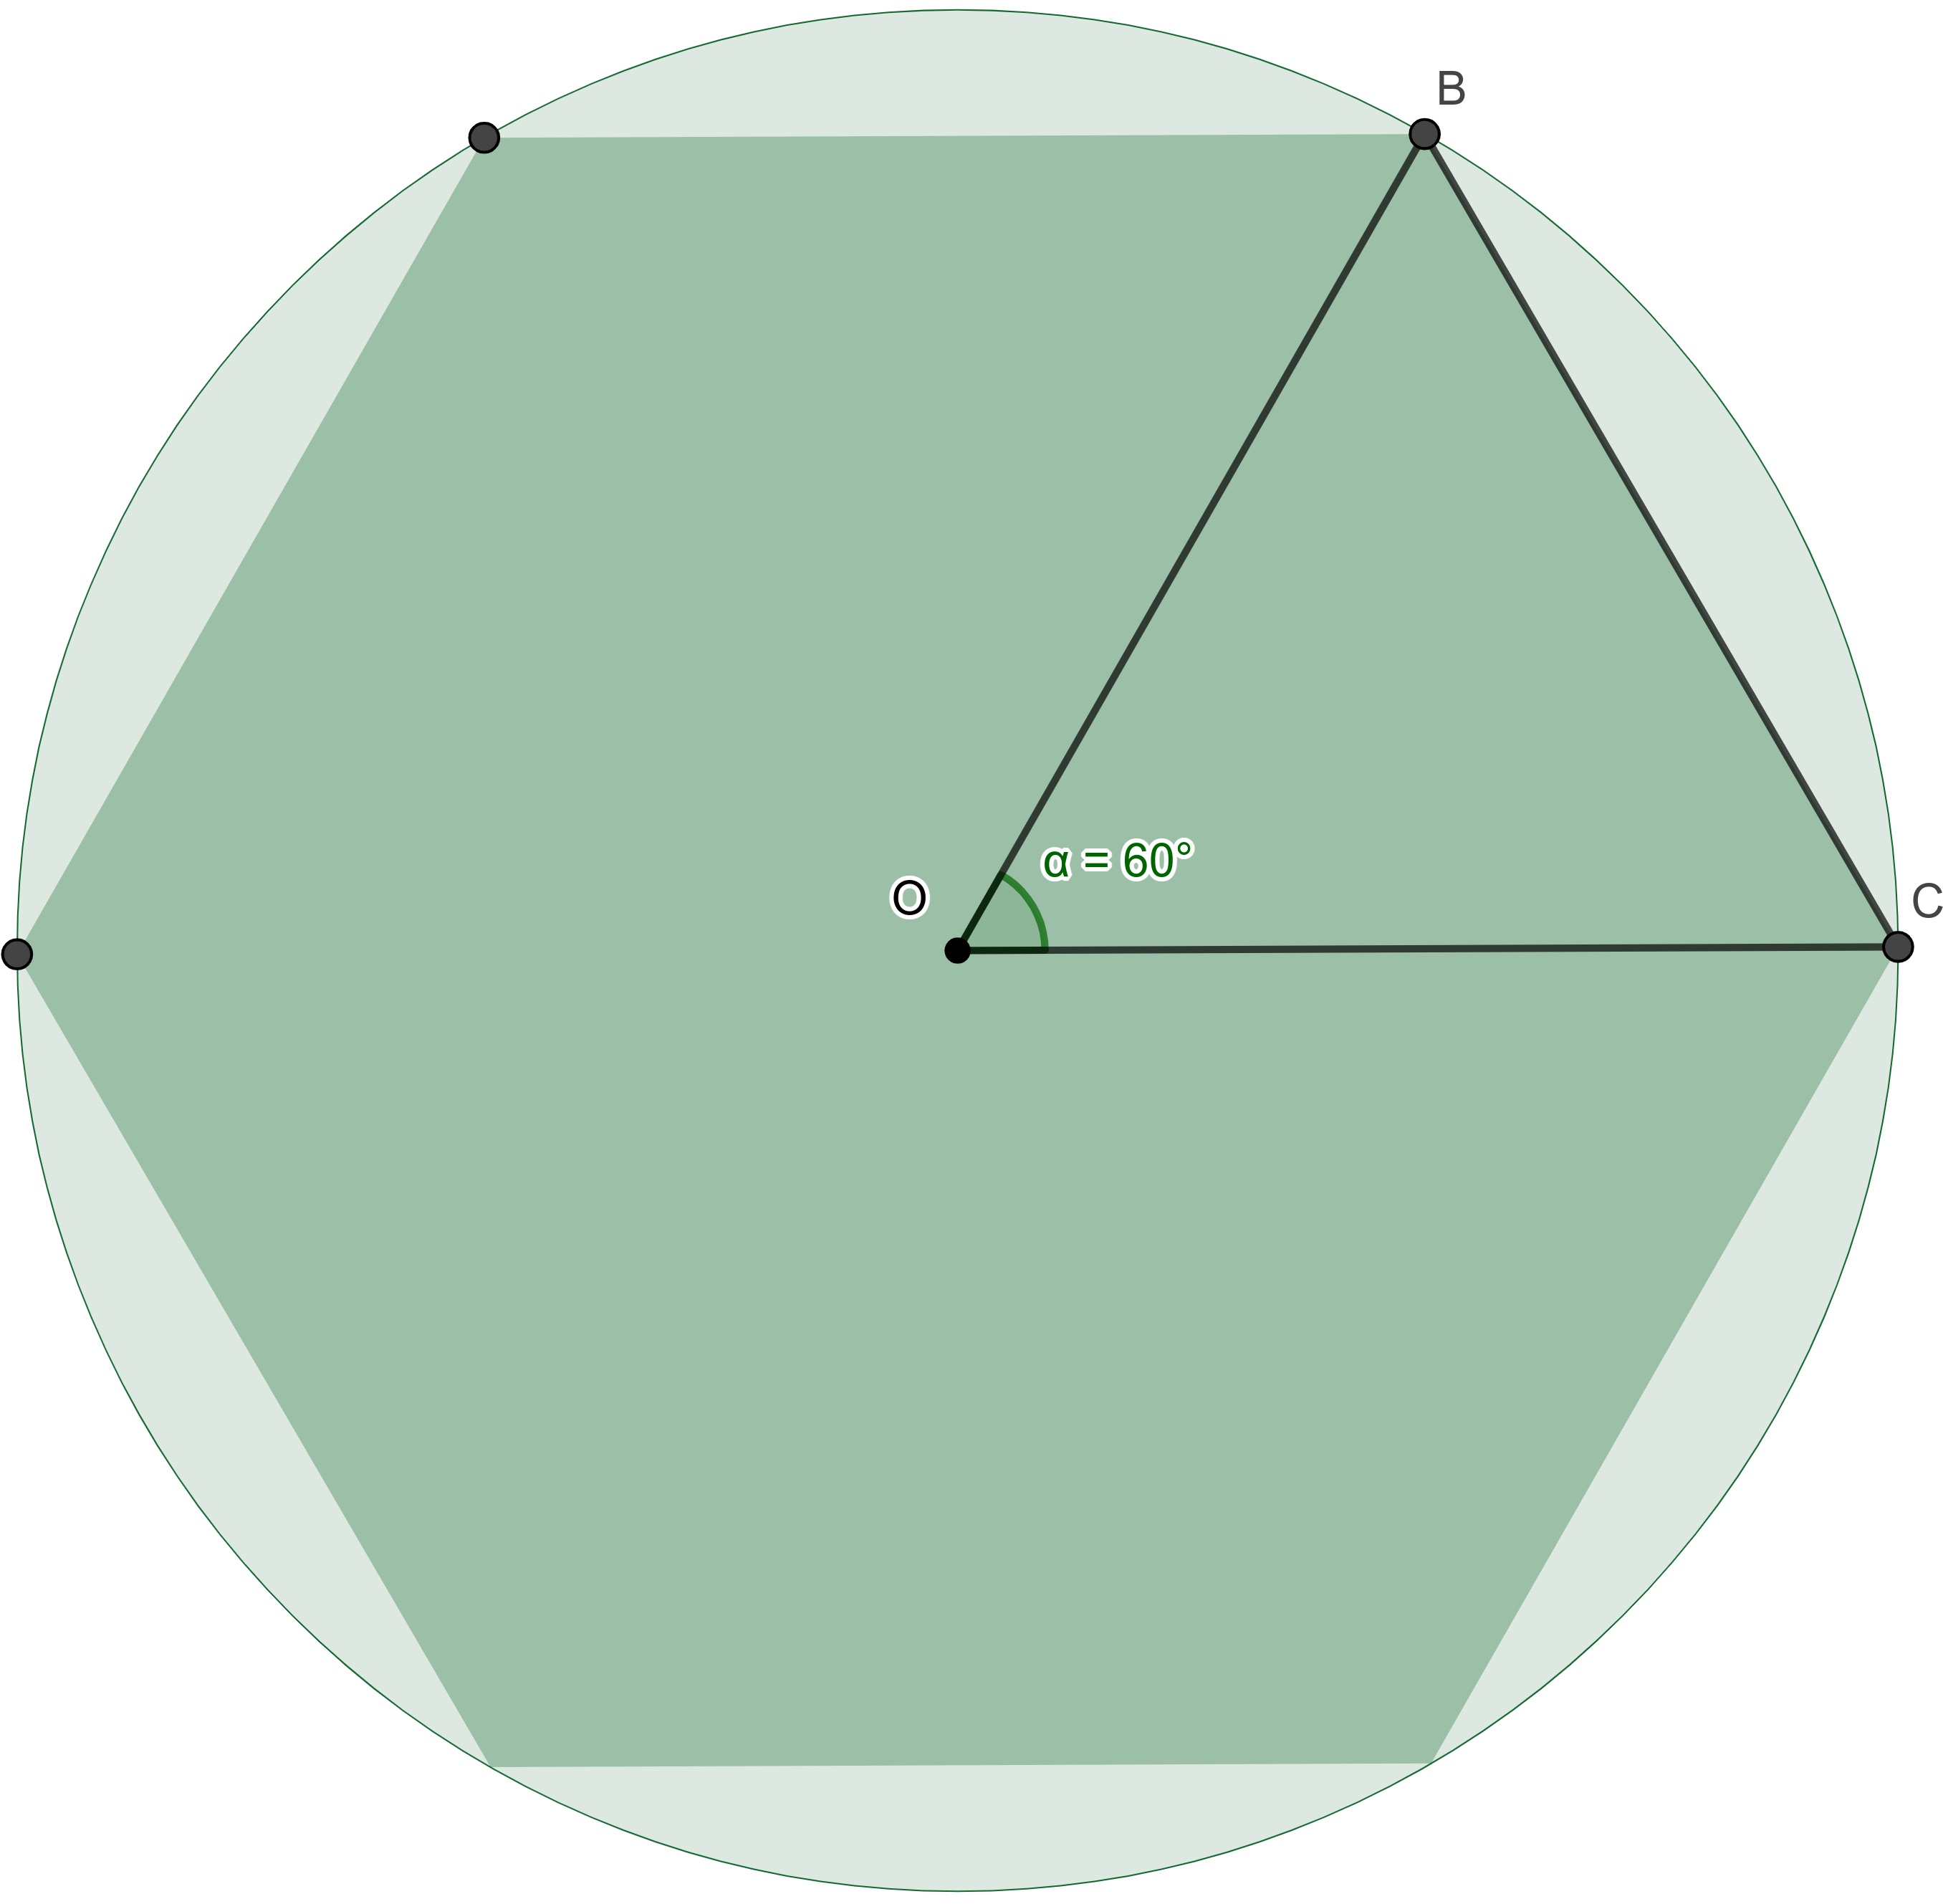
\includegraphics[height=3.3cm]{img/fig2_copy.png}
		\end{center}
		\pause
		\begin{block}{}
			A medida que aumentamos el número de nodos del polígono $P_n$ se aproxima, cada vez más, al círculo. Obteniendo una forma de calcular el área mediante subdivisiones.
			$$A_{\text{círculo}}=\lim_n A_{P_n} $$
		\end{block}
	\end{frame}
	\begin{frame}
		\begin{block}{}
			Esta misma idea se puede llevar casi a cualquier área, en este caso el área bajo la curva de la función $f(x)=x^2, \forall x\geq0$
		\end{block}
		\ \\
		\begin{center}
			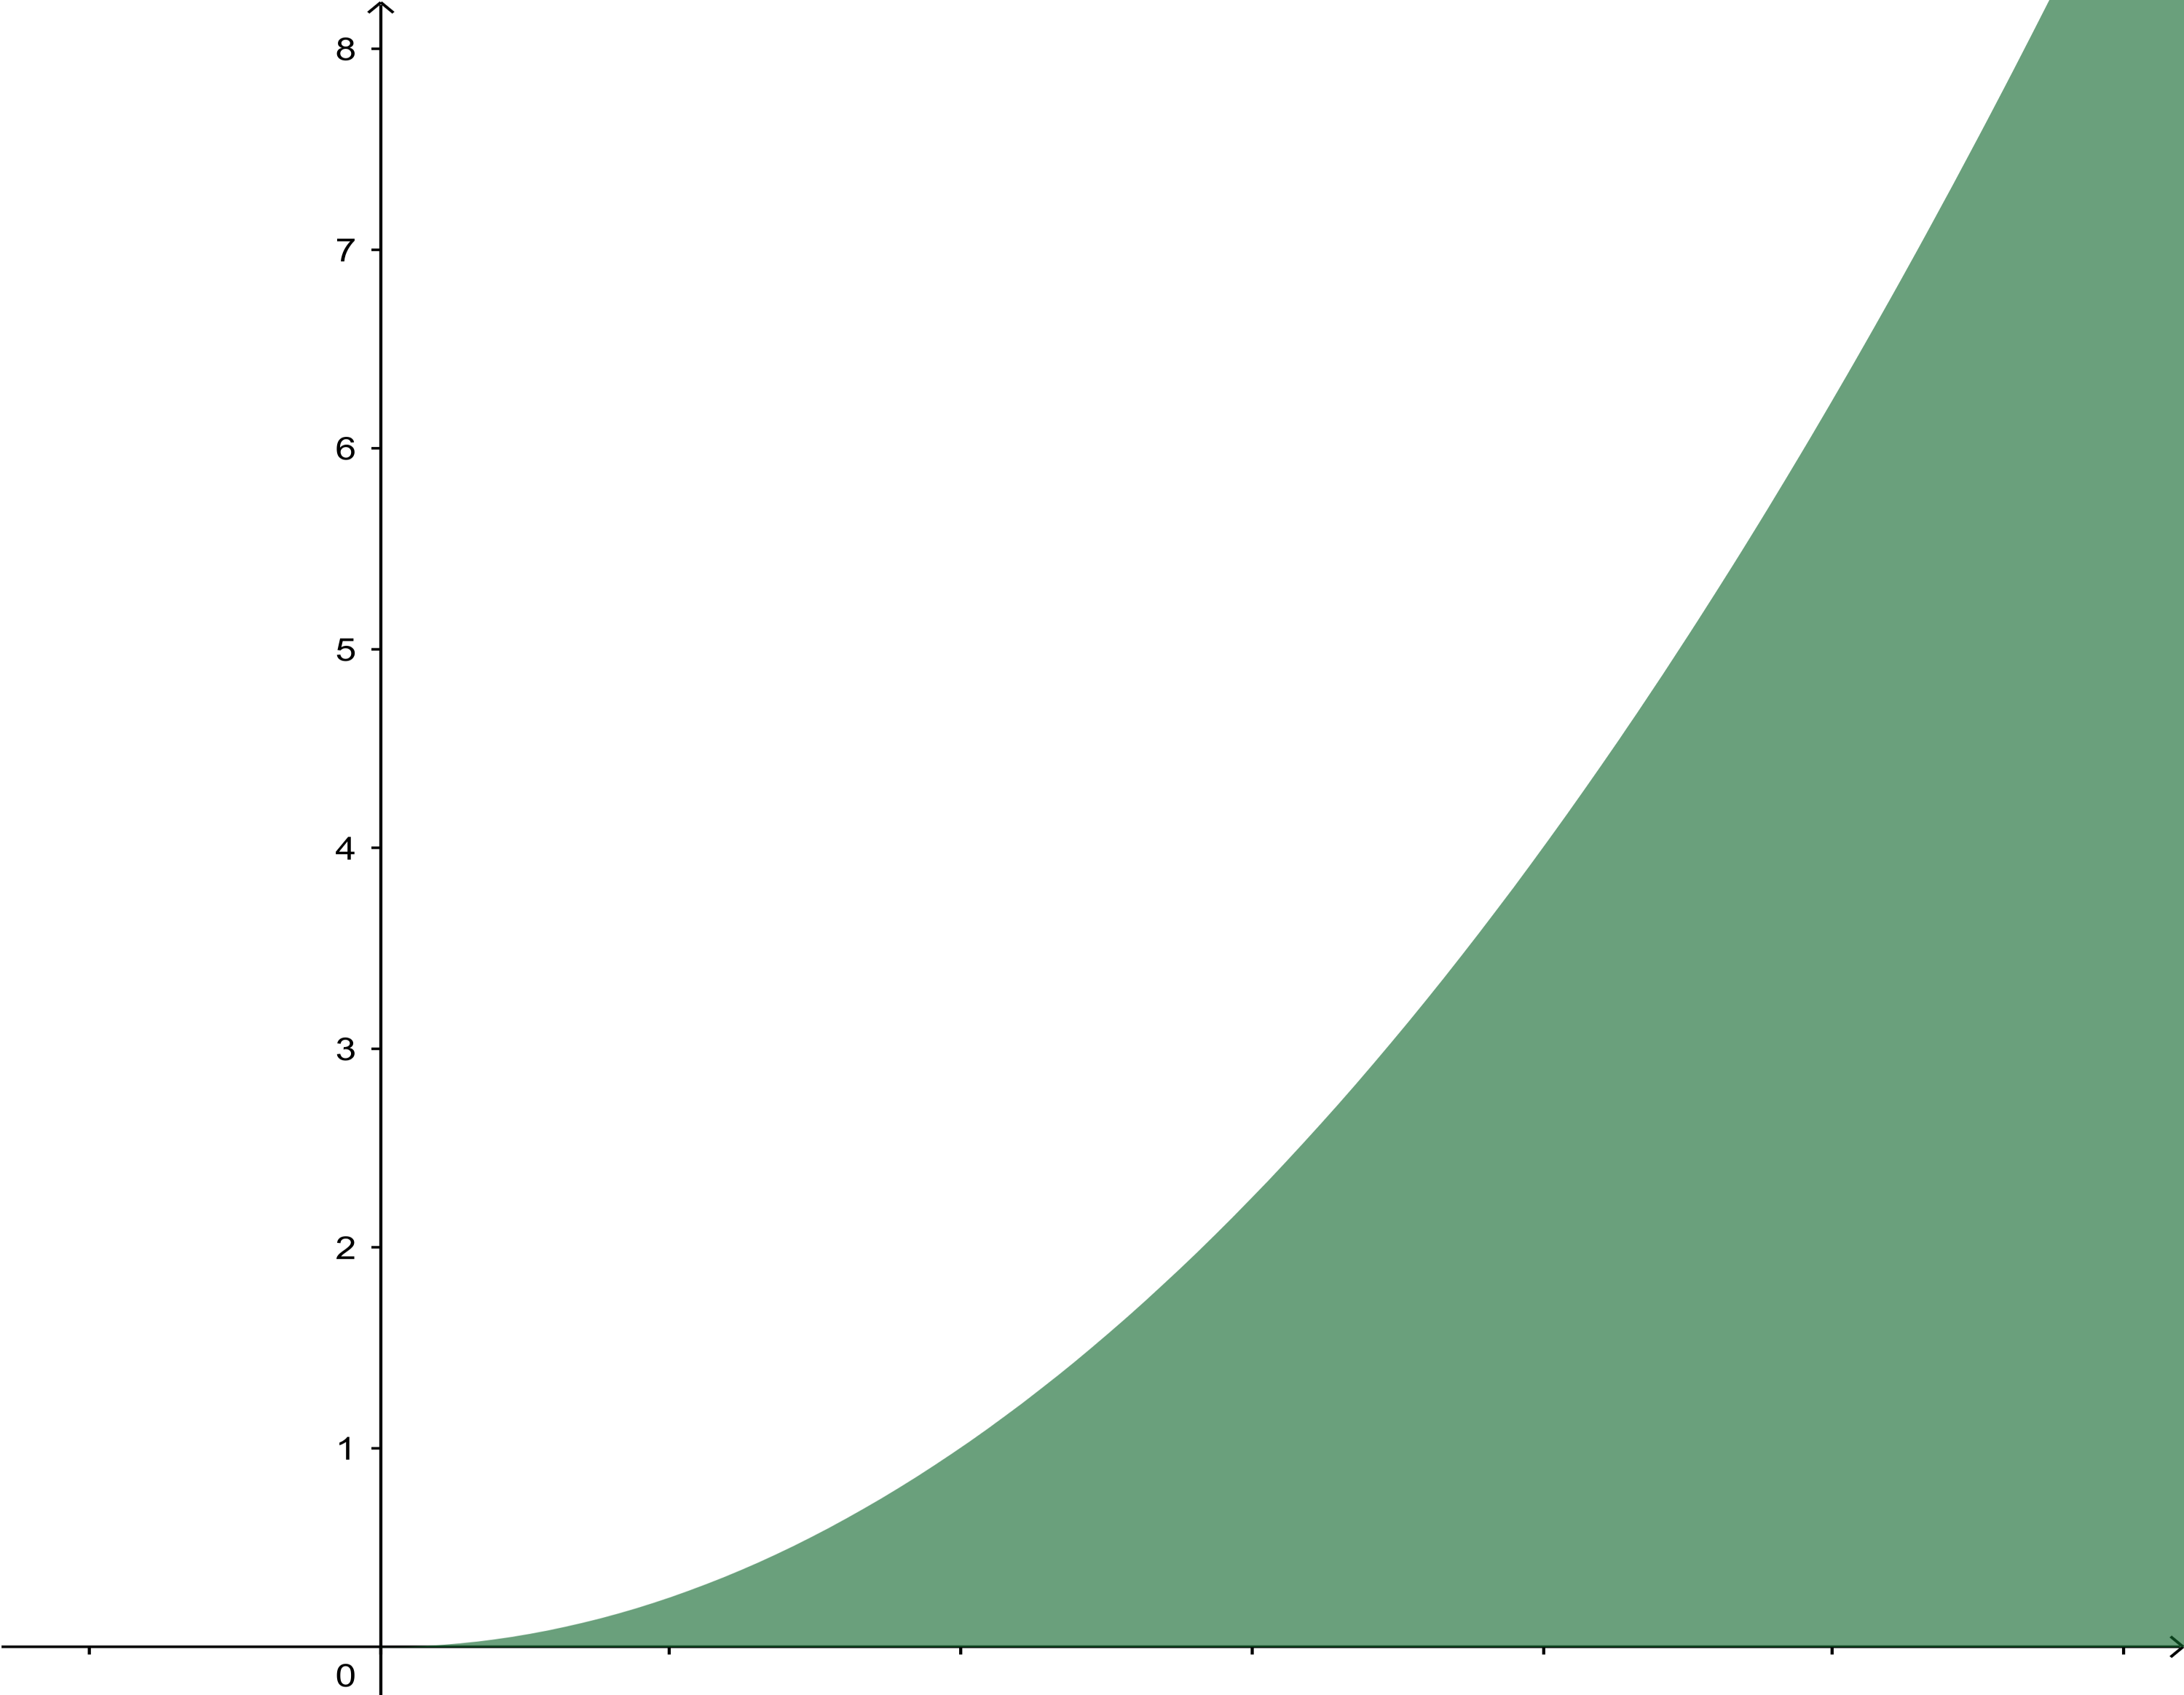
\includegraphics[height=5cm]{img/fig3_p.png}
		\end{center}
	\end{frame}
	\begin{frame}
		\begin{block}{}
			Esta misma idea se puede llevar casi  a cualquier área, en este caso el área bajo la curva de la función $f(x)=x^2, \forall x\geq0$
		\end{block}
		\ \\
		\begin{center}
			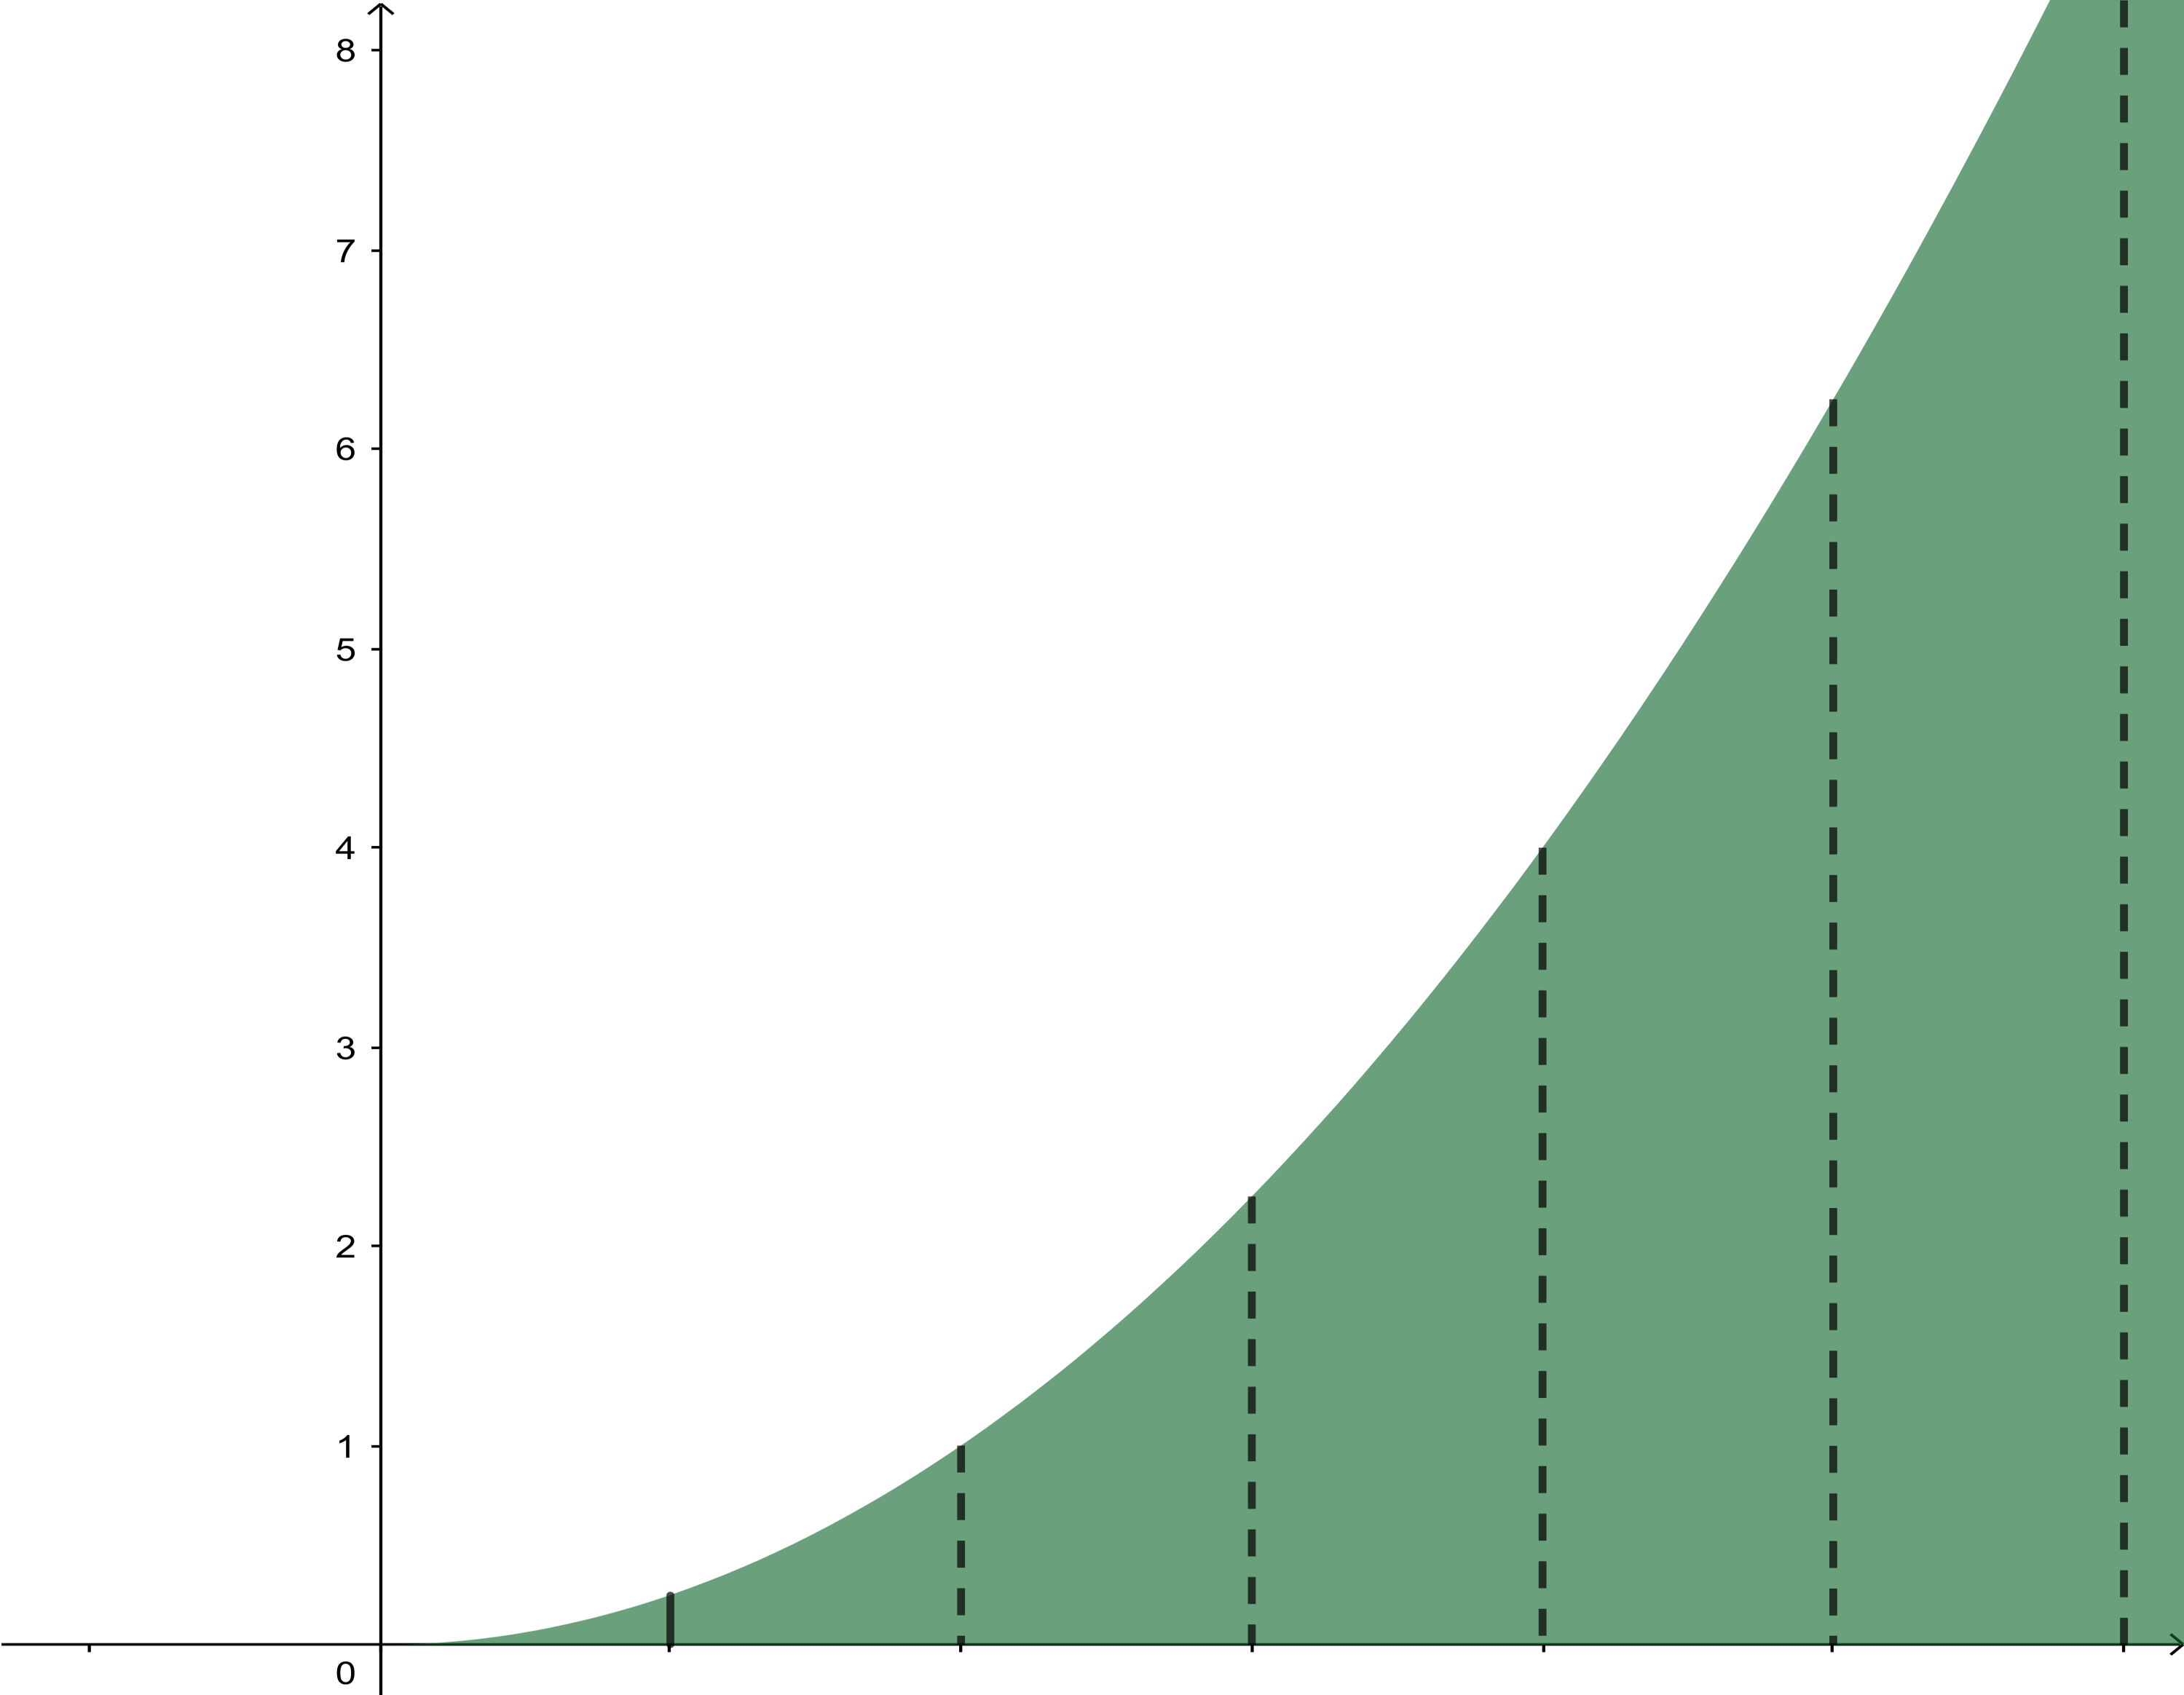
\includegraphics[height=5cm]{img/fig4_p.png}
		\end{center}
	\end{frame}
	\begin{frame}
		\begin{block}{}
			Esta misma idea se puede llevar casi a cualquier área, en este caso el área bajo la curva de la función $f(x)=x^2, \forall x\geq0$
		\end{block}
		\ \\
		\begin{center}
			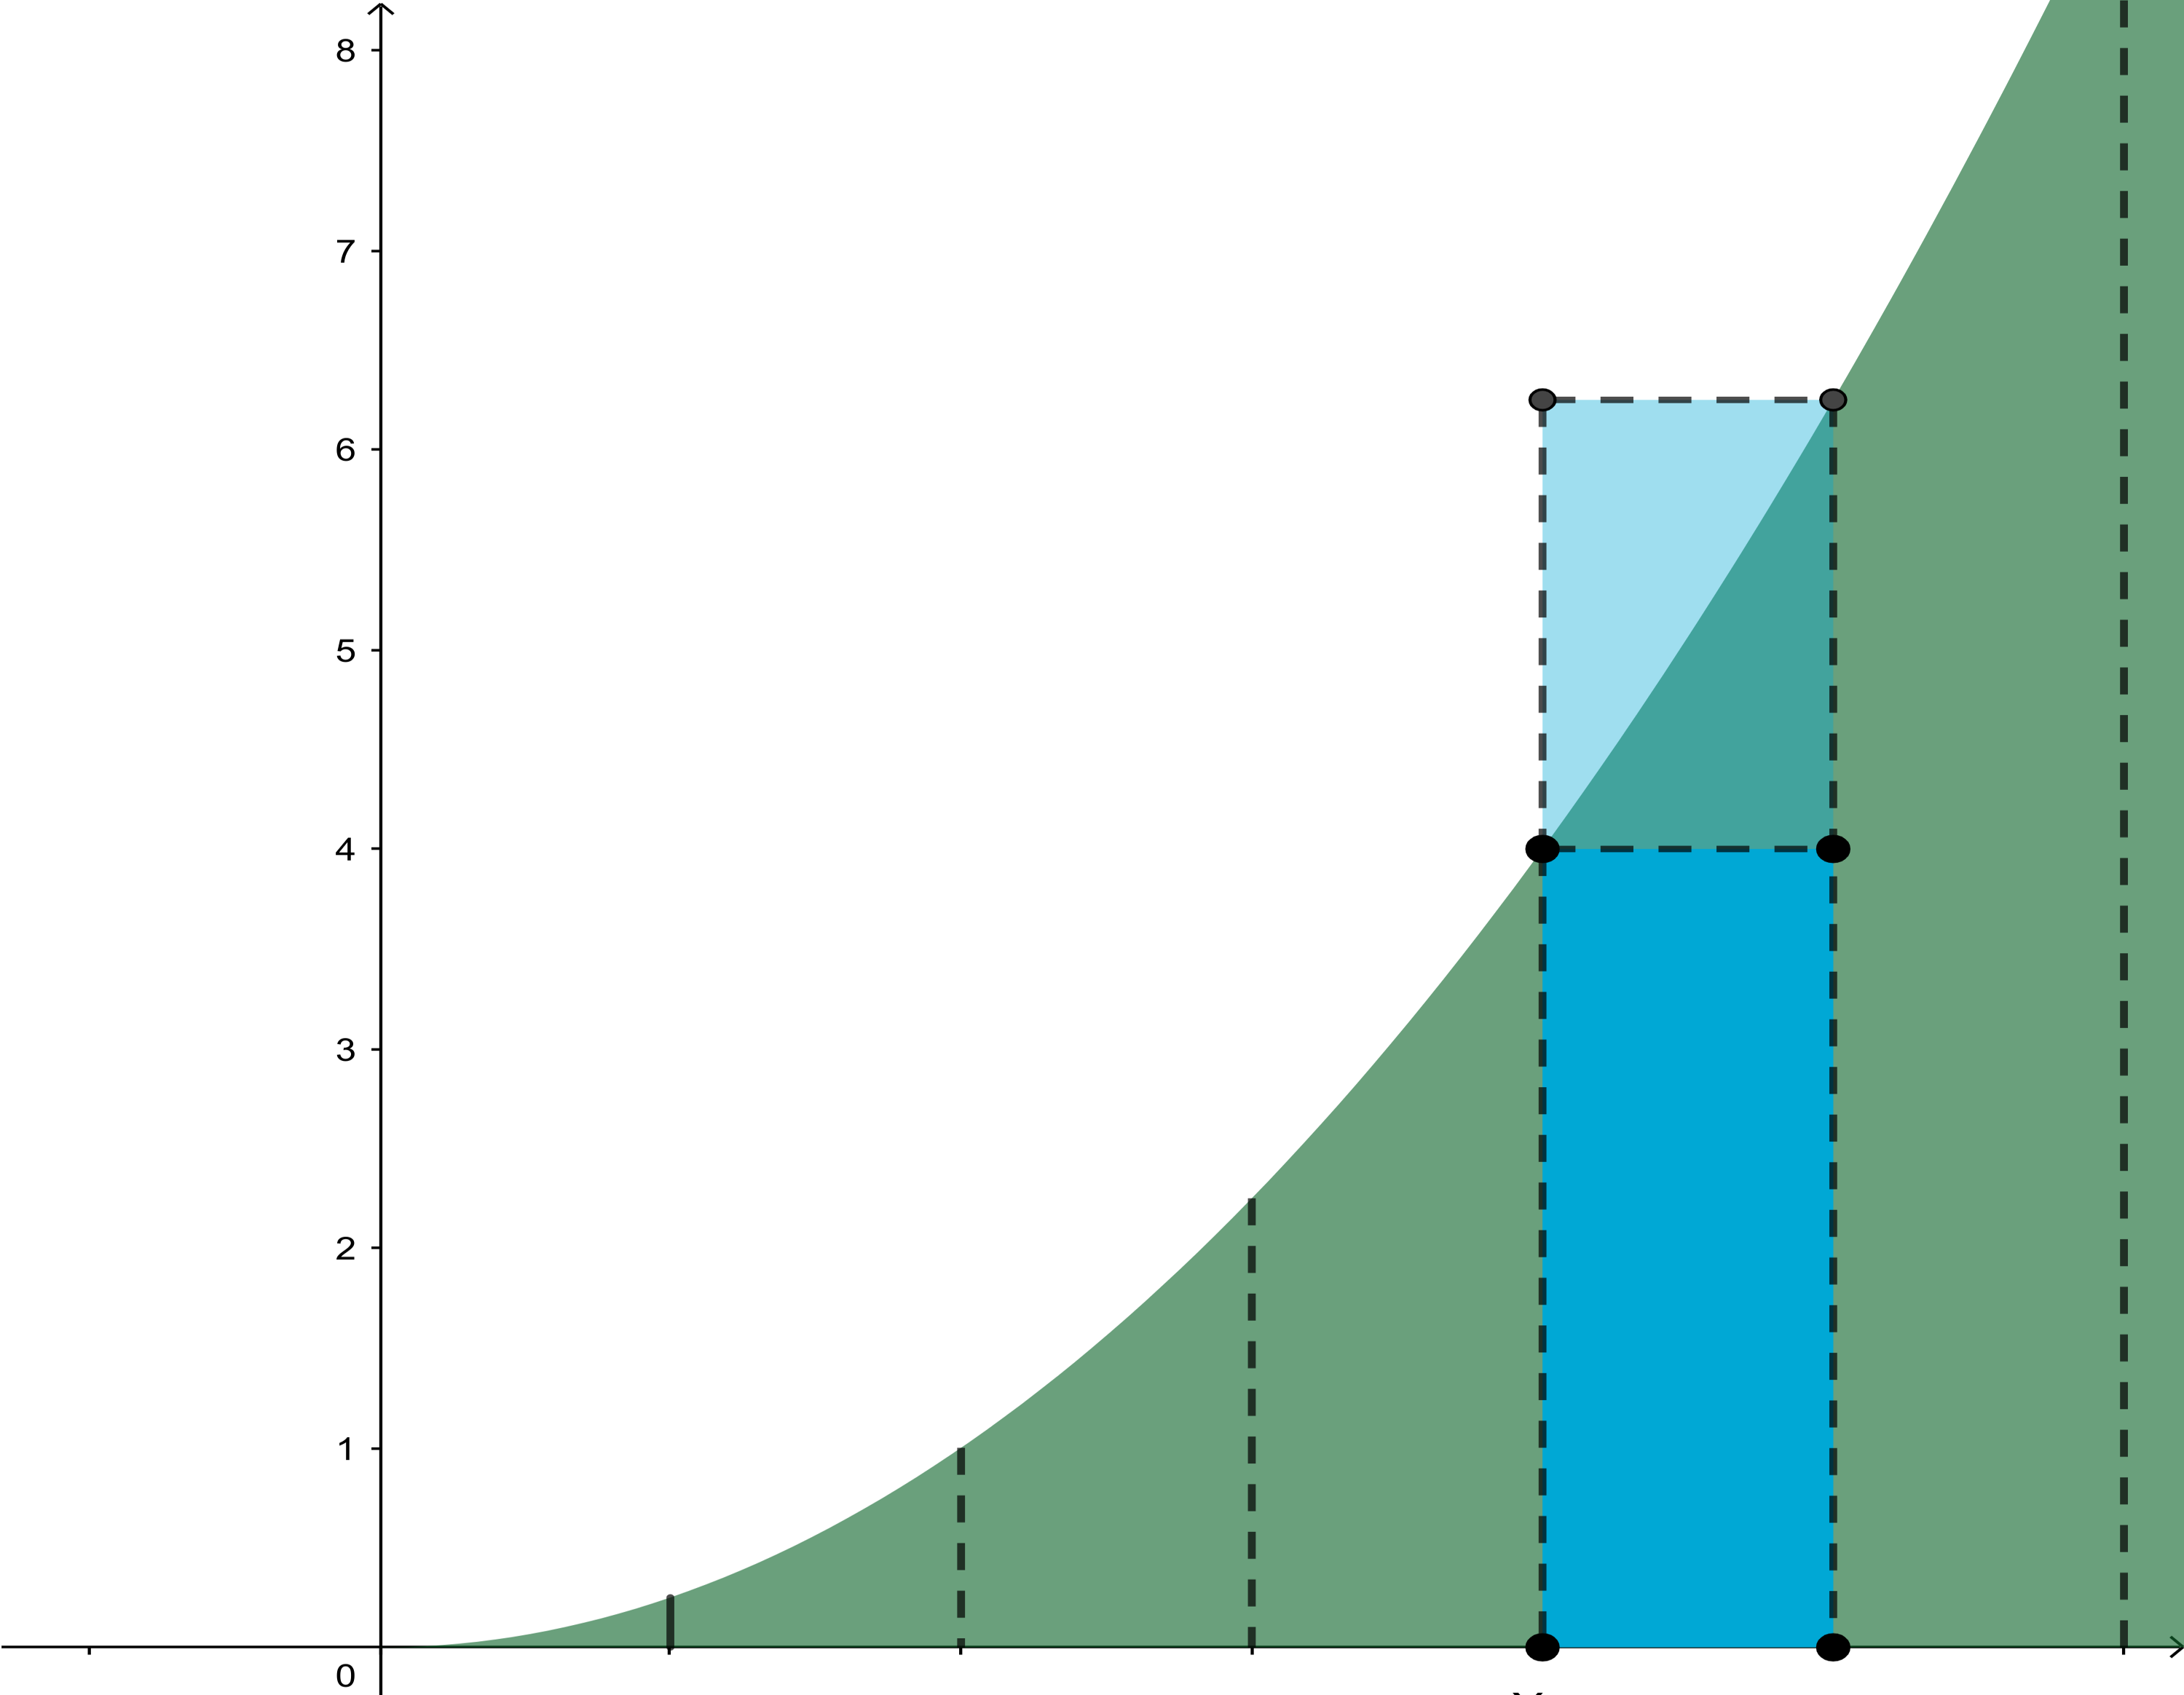
\includegraphics[height=5cm]{img/fig5_p.png}
		\end{center}
	\end{frame}
	\begin{frame}
		\begin{block}{Definición}
			Dado una partición $p$, llamaremos Sunma Superior de Darboux a la suma de las áreas de los rectángulos superiores.
			$$S_p=\sum_{i=0}^nM_i\Delta x_i$$
			donde $M_i=\sup_{[x_{i-1},x_i]}f(x)$
			y de igual manera, llamaremos Suma Inferior de Darboux a la suma de las áreas de los rectángulos inferiores.
			$$s_p=\sum_{i=0}^nm_i\Delta x_i$$
			donde $m_i=\inf_{[x_{i-1},x_i]}f(x)$
		\end{block}
		\pause
		A medida que aumentamos el número de subdivisiones de la partición estas sumas se van aproximando cada vez más a una función con ``área''
	\end{frame}
	\begin{frame}
		\ \\ \ \\
		\begin{block}{Definición}
			Llamaremos integral de una función $f$, $I(f)=\int f(x)dx$ al área bajo la curva de la función $f$. Y se cumple que $s_p^f\leq I(f)\leq S_p^f$.
		\end{block}
		\pause
		A medida que $\Delta x_i\rightarrow 0$, $\lvert s_p-S_p\rvert\rightarrow 0$, luego por el teorema del emparedado obtendríamos que cuando $\Delta x_i\rightarrow 0$, $s_p^f=I(f)=S_p^f$. Por consiguiente, podemos definir:
		\pause
		\begin{block}{Definición}
			Diremos que una función es Darboux integrable si $\exists \lim\limits_{\Delta x_i\rightarrow 0}\lvert S_p-s_p\rvert$ y además $\lim\limits_{\Delta x_i\rightarrow 0}\lvert S_p-s_p\rvert=0$
		\end{block}
	\end{frame}
	\begin{frame}
		\begin{block}{Definición}
			Llamaremos suma {\it integral de Riemann} de $f$ respecto a la partición  $P$ a:
		$$\sigma_f(P,\eta_i)=\sum_{i=1}^nf(\eta_i)\Delta x_i,\ \text{con}\ \eta\in[x_{i-1},x_i], (i=1,2,...,n)$$
		\end{block}
		\pause
		\begin{block}{}
			Diremos que $f$ es integrable según Riemann en un compacto, si existe:
		$$I=\lim_{\lambda(P)\rightarrow 0}\sigma_f(P,\eta_i)$$
		\end{block}
		\pause
		\begin{block}{Teorema}
			Como:
			$$s_p\leq \sigma(P,\eta)\leq S_p,\ \forall P$$
			entonces $f$ es Darboux Integrable $\Leftrightarrow$ $f$ es Riemann Integrable.
		\end{block}
	\end{frame}
	\begin{frame}
		\begin{block}{Teorema:}
			Toda función continua en un intervalo $[a,b]$ es Riemann integrable en $[a,b]$.	
		\end{block}
		\pause
		\begin{block}{Colorario:}
			Si una función $f$ tiene sólo un número finito de discontinuidades (tipo salto o evitable) en $[a, b]$, entonces $f$ es Riemann-integrable en $[a, b]$.			
		\end{block}
	\end{frame}
	\begin{frame}
		\begin{block}{Teorema:}
			Toda función continua en un intervalo $[a,b]$ es Riemann integrable en $[a,b]$.	
		\end{block}
		\begin{block}{Colorario:}
			Si una función $f$ tiene sólo un número finito de discontinuidades (tipo salto o evitable) en $[a, b]$, entonces $f$ es Riemann-integrable en $[a, b]$.			
		\end{block}
		\begin{center}
			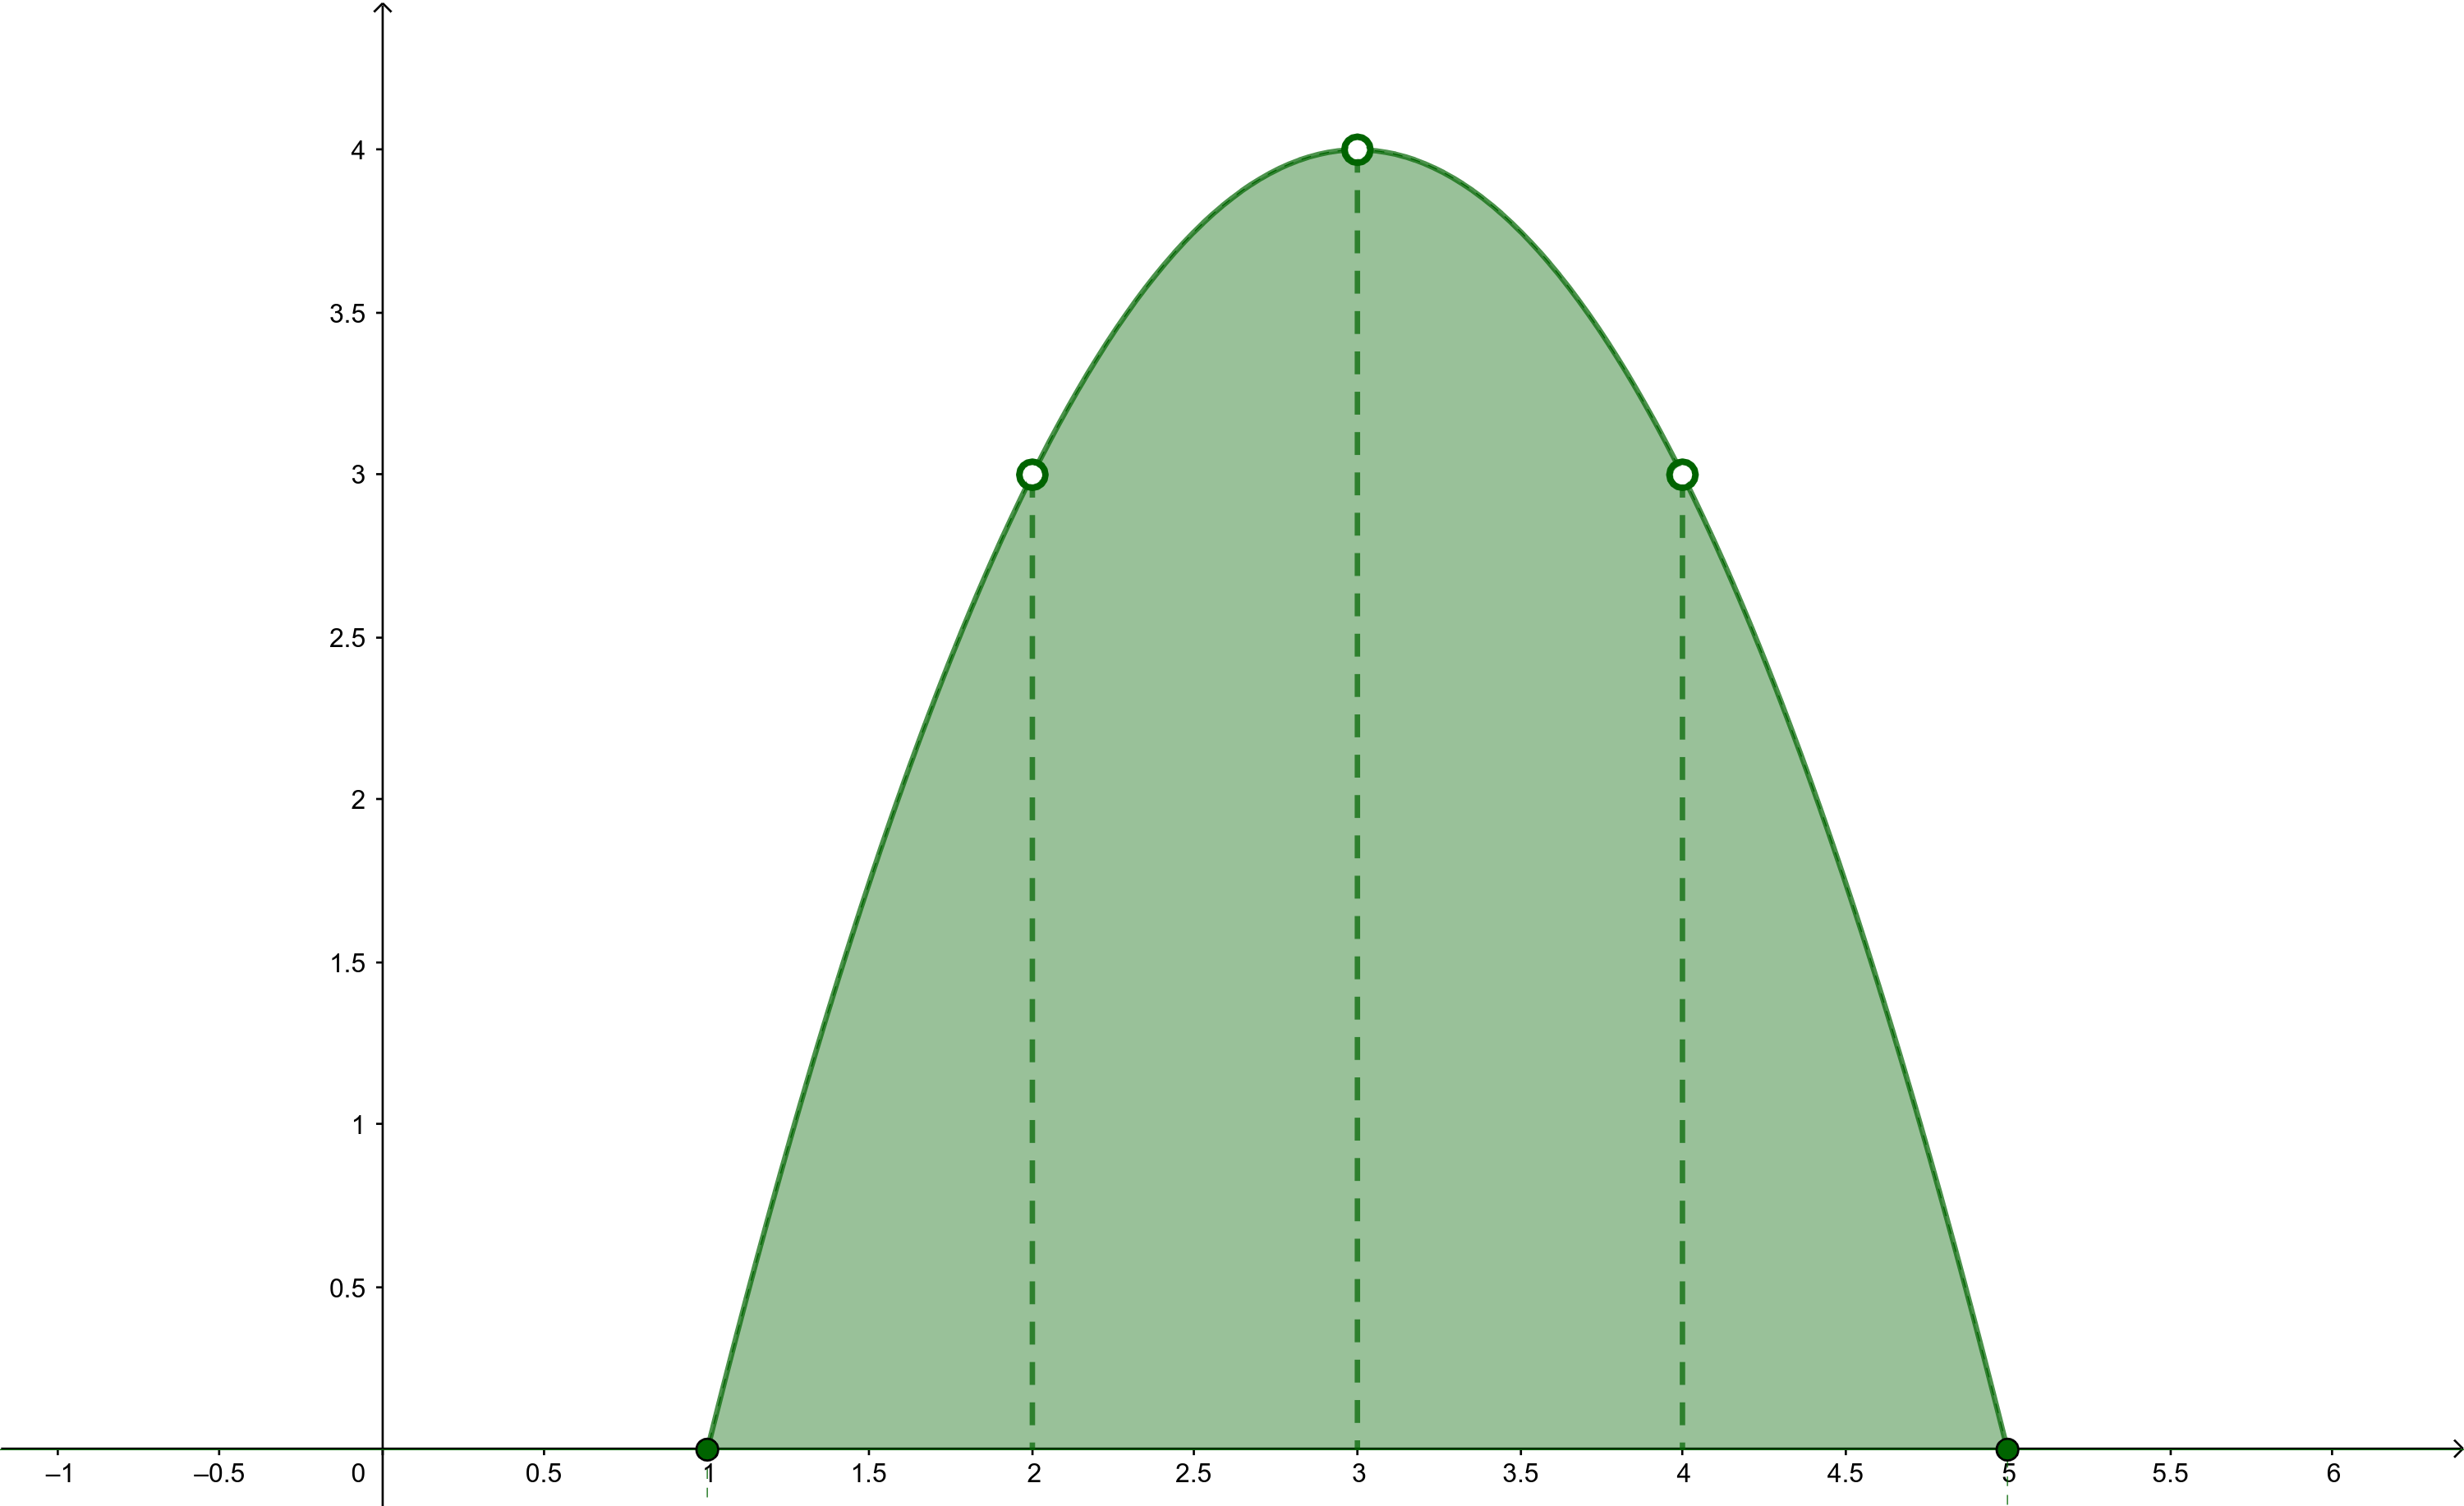
\includegraphics[height=5cm]{img/discontinuidades.png}
		\end{center}
	\end{frame}
	\begin{frame}
		A partir de la definción se pueden obtener algunas propiedades fundamentales del cálculo integral.
		\begin{block}{}
			\begin{enumerate}[<+->]
				\item Sean $f$,$g\in R[a,b]$ y $\alpha,\beta\in\mathbb{R}\Rightarrow \alpha f+\beta g\in R[a,b]$ y se cumple que:
				$$\int_a^b(\alpha f+\beta g)(x)dx=\alpha\int_a^b f(x)dx+\beta\int_a^bg(x)dx$$
				\item Si $f\in R[a,b]$ y $[\alpha,\beta]\subset[a,b]\Rightarrow f\in R[\alpha,\beta]$
				\item Si $a<c<b$, $f\in R[a,c]$ y $f\in R[c,b]\Rightarrow f\in R[a,b]$ y se cumple:
				$$\int_a^b f(x)dx=\int_a^cf(x)dx+\int_c^bf(x)dx$$
				\item Si $\displaystyle f\in R[a,b],\ f(x)\geq 0, \forall x\in[a,b]\Rightarrow \int_a^bf(x)dx\geq0$
				\item Sean $\displaystyle f,g\in R[a,b],\ f(x)\leq g(x)\ \forall x\in[a,b]\Rightarrow \int_a^bf(x)dx\leq\int_a^bg(x)dx$
			\end{enumerate}
		\end{block}
	\end{frame}
	\begin{frame}
		\begin{block}{Integrales Inmediatas}
			\begin{itemize}[<+->]
				\item $\displaystyle \int 0dx=c$, donde $c\in\mathbb{R}$
				\item Sea $a\in\mathbb{R}$ y $n\in\mathbb{Z}, n\neq-1\Rightarrow$ $\displaystyle \int ax^ndx=\dfrac{a}{n+1}x^{n+1}+c$, donde $c\in\mathbb{R}$
				\item $\displaystyle\int\dfrac{1}{x}dx=ln(x)+c$, donde $c\in\mathbb{R}$
				\item $\displaystyle\int e^x=e^x+c$, donde $c\in\mathbb{R}$
				\item Sea $\displaystyle a\in\mathbb{R}, a>0\Rightarrow \int a^xdx=\dfrac{a^x}{\ln a}+c$, donde $c\in\mathbb{R}$
				\item $\displaystyle \int\cos(x)dx=\sin(x)dx+c$, donde $c\in\mathbb{R}$
				\item $\displaystyle \int\sin xdx=-\cos xdx+c$, donde $c\in\mathbb{R}$
			\end{itemize}
		\end{block}
	\end{frame}
	\begin{frame}
		\begin{block}{}
			\begin{itemize}[<+->]
				\item $\displaystyle \int\dfrac{1}{\cos^2 x}dx=\tan x+c$, donde $c\in\mathbb{R}$
				\item $\displaystyle \int-\dfrac{1}{\sin^2 x}dx=\text{cot}\ x+c$, donde $c\in\mathbb{R}$
			\end{itemize}
		\end{block}
		\pause[3]
		{\bf Ejemplo 1:} Calcula la integral indefinida:
			$$\displaystyle \int (3\sin(x)+x)dx$$
			\pause[4]
			\begin{align*}
				\int (3\sin(x)+x)dx&=\int 3\sin(x)dx+\int xdx=3\int\sin(x)dx+\int xdx\\
				&=-3\cos(x)+c_1+\dfrac{x^2}{2}+c_2\\
				&=-3\cos(x)+\dfrac{x^2}{2}+C
			\end{align*}
	\end{frame}
	\begin{frame}
		{\bf Ejemplo 2:} Calcula la integral indefinida:
		$$\displaystyle \int \dfrac{\sin(2x)}{\cos(x)}dx$$
		\pause
		Sabemos de trigonometría que:
		$$\sin(2x)=2\sin(x)\cos(x)$$
		luego:
		\begin{align*}
			\int \dfrac{\sin(2x)}{\cos(x)}dx&=\int\dfrac{2\sin(x)\cos(x)}{\cos(x)}dx\\
			&=\int2\sin(x)dx\\
			&=2\int\sin(x)dx\\
			&=-2\cos(x)+c
		\end{align*}
	\end{frame}
	\begin{frame}
		{\bf Ejercicios de estudio independiente}
		\begin{center}
			Calcule las siguientes integrales:
			\begin{enumerate}
				\item[a$)$] $\displaystyle \int\dfrac{2}{x^3}dx$
				\item[b$)$] $\displaystyle \int\sqrt{1-\sin^2(x)}dx$
				\item[c$)$] $\displaystyle \int (x^4+3x^2+5)dx$
				\item[d$)$] $\displaystyle \int \left(e^x+\dfrac{1}{x}\right)dx$
			\end{enumerate}
		\end{center}
	\end{frame}
\end{document}